\section{Theorie}
\label{sec:Theorie}
Bei Anwesenheit von Materie hängen magnetische FLussdichte $\symbf{B}$, externe
magnetische Feldstärke $\symbf{H}$, magnetische Permeabilität des Vakuums $\mu_0$
und Magnetisierung des Materials $\symbf{M}$ durch
\begin{equation}
  \symbf{B} = \mu_0 \symbf{H} + \symbf{M}
  \label{eqn:bhm}
\end{equation}
zusammen. Die Magnetisierung $\symbf{M}$ beschreibt hierbei die Dichte der
magnetischen Dipolmomente im Material und hängt durch
\begin{equation}
  \symbf{M} = \mu_0 \chi \symbf{H}
  \label{eqn:mchih}
\end{equation}
von dem externen Magnetfeld $\symbf{H}$ ab. Dabei ist die Proportionalitätskonstante
$\chi$ die magnetische Suszeptibilität. Im einfachsten Fall ist sie eine materialabhängige
Konstante, kann aber im allgemeinen Fall vom externen Magnetfeld und der Temperatur $T$
des Materials abhängen.
In diesem Versuch wird die Suszeptibilität paramagnetischer Substanzen untersucht.
Nur Atome, Moleküle oder Ionen mit nicht verschwindendem Drehimpuls weisen
Paramagnetismus auf. Dieser beruht darauf, dass sich magnetische Momente parallel zu
einem äußeren Magnetfeld ausrichten. Da thermische Bewegungen dies stören, ist der Effekt
temperaturabhängig. Da der atomare Drehimpuls mit dem magnetischen Moment gekoppelt ist,
soll dieser Zusammenhang erläutert werden.
Der Gesamtdrehimpuls $\symbf{J}$ eines Atoms setzt sich aus dem Bahndrehimpuls
$\symbf{L}$ der Elektronenhülle, dem Eigendrehimpuls, dem sogenannten Spin, $\symbf{S}$
und dem Kernspin, der für paramagnetische Effekte vernachlässigt werden kann, zusammen.
Unter die Voraussetzung eines nicht zu starken Magnetfeldes addieren sich beide
Drehimpulse zu einem Gesamtdrehimpuls $\symbf{J}$ durch
\begin{equation}
  \symbf{J} = \symbf{L} + \symbf{S}\,.
  \label{eqn:ls}
\end{equation}
Es kann angenommen werden, dass sich $\symbf{L}$ und $\symbf{S}$ als ungewichtete
Summe der einzelnen Bahndrehimpulse $\symbf{l}_i$ und Spins $\symbf{s}_i$ ergeben.
Die Addition zu einem Gesamtdrehimpuls wird als LS-Kopplung bezeichnet. Für die
resultierenden magnetischen Momente gilt dann
\begin{align}
  \symbf{\mu_L} &= - \frac{\mu_B}{\hbar} \symbf{L} \,\\
  \symbf{\mu_S} &= - g_S \frac{\mu_B}{\hbar} \symbf{S} \,.
  \label{eqn:mulmus}
\end{align}
Dabei bezeichnet $\mu_B$ das Bohrsche Magneton und $\hbar$ das reduzierte Plancksche
Wirkungsquantum.
Allgemein gilt die Relation
\begin{equation}
  |\symbf{N}| = \sqrt(N(N+1)) \hbar
\end{equation}
für einen der drei Drehimpulse als $\symbf{N}$ mit seiner dazugehörigen Quantenzahl
$N$. Damit ergeben sich die Beträge der magnetischen Momente zu
\begin{align}
  |\symbf{\mu_L}| &= \mu_B \sqrt{L(L+1)} \, \label{eqn:absmul}\\
  |\symbf{\mu_S}| &= g_S \mu_B \sqrt{S(S+1)} \, \label{eqn:absmus}.
  \label{eqn:absmulmus}
\end{align}
Dabei ist $L$ die Bahndrehimpulsquantenzahl und $S$ die Spinquantenzahl.
Mit $\symbf{\mu}_J$ sei der zu $\symbf{J}$ parallele Anteil des zum Gesamtdrehimpuls $\symbf{J}$
gehörigen magnetischen Moments $\symbf{\mu}$ bezeichnet.

\begin{figure}
  \centering
  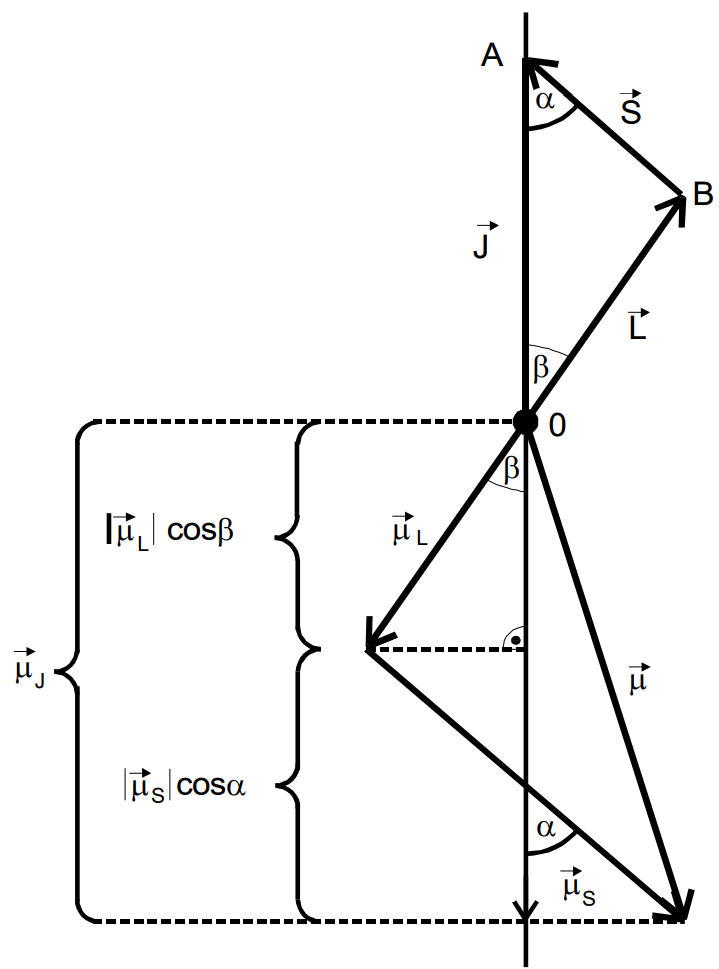
\includegraphics[width=180pt]{data/drehimpulse.png}
  \caption{Vektorielle Veranschaulichung zu den atomaren Drehimpulsen und den magnetischen Momenten \cite{Versuchsanleitung}}
  \label{fig:vektordreh}
\end{figure}

Aus Abbildung \ref{fig:vektordreh} lässt sich die Beziehung
\begin{equation}
  |\symbf{\mu}_J| = |\symbf{\mu}_S| \cos(\alpha) + |\symbf{\mu}_L| \cos(\beta)\,.
  \label{eqn:cos}
\end{equation}
Mithilfe des Kosinussatzes und dem Einsetzen der Gleichungen \ref{eqn:absmul} und \ref{eqn:absmus} in Gleichung
\ref{eqn:cos}
